\documentclass[10pt]{article}
\usepackage[polish]{babel}
\usepackage[utf8]{inputenc}
\usepackage[T1]{fontenc}
\usepackage{amsmath}
\usepackage{amsfonts}
\usepackage{amssymb}
\usepackage[version=4]{mhchem}
\usepackage{stmaryrd}
\usepackage{graphicx}
\usepackage[export]{adjustbox}
\graphicspath{ {./images/} }
\usepackage{hyperref}
\hypersetup{colorlinks=true, linkcolor=blue, filecolor=magenta, urlcolor=cyan,}
\urlstyle{same}

\title{Zadania - etap I }

\author{}
\date{}


\begin{document}
\maketitle
(klasy 7 i 8 szkoły podstawowej i klasa III gimnazjum)

Zadanie 1. Oblicz wartość liczby: \(a=\sqrt{1+2004 \cdot \sqrt{1+2003 \cdot \sqrt{1+2002 \cdot \sqrt{1+2001 \cdot 1999}}} .}\).\\
Zadanie 2. Oblicz wartość wyrażenia \(\frac{a+b}{a-b}\), jeśli wiadomo, że liczby \(a, b\) spełniają równość:

\[
2 a^{2}+4 a b=a b+2 b^{2} .
\]

Zadanie 3. Ile wynosi różnica pól figury \(F_{1}\) (Rys. a)) i figury \(F_{2}\) (Rys. b)), jeśli bok kwadratu ABCD ma długość 10 cm ?\\
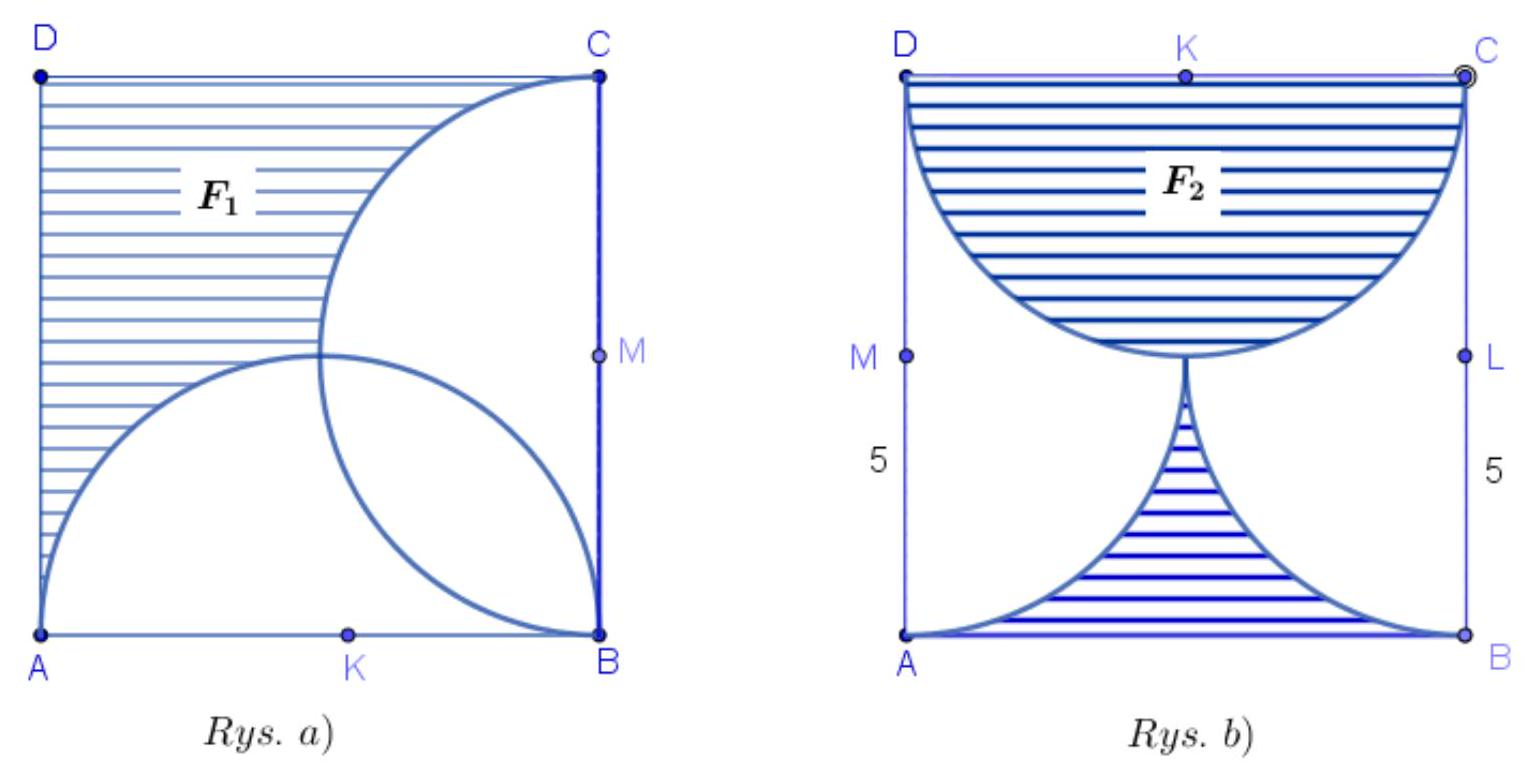
\includegraphics[max width=\textwidth, center]{2024_11_21_217d24491fe826e256c5g-1}

Zadanie 4. Rozwiąż równanie \(||||x|-1|-2|-3|-4 \mid=0\).

Zadanie 5. Suma dwóch ułamków wynosi \(\frac{53}{80}\). Liczniki tych ułamków są w stosunku 5: 7, a mianowniki w stosunku 4:5. Znajdź te ułamki.

CENTRUM NAUCZANIA MATEMATYKI I KSZTALCENIA NA ODLEGLOŚĆ

\section*{ZAŁACZNIK DO KARTY UCZESTNIKA KONKURSU „OD SZKOLNIAKA DO ŻAKA"}
\section*{Oświadczenie}
Zgodnie z art. 6 ust. 1 lit. a ogólnego rozporządzenia o ochronie danych osobowych z dnia 27 kwietnia 2016 r. (Dz. Urz. UE L 119 z 04.05.2016) (RODO) oświadczam, że wyrażam zgodę na przetwarzanie przez Politechnikę Gdańską z siedzibą w Gdańsku, ul. Narutowicza 11/12, 80-233 Gdańsk, danych osobowych mojego dziecka w celu i zakresie niezbędnym do przeprowadzenia konkursu „Od szkolniaka do żaka".

\section*{Klauzula informacyjna}
Zgodnie z art. 13 ogólnego rozporządzenia o ochronie danych osobowych z dnia 27 kwietnia 2016 r. (Dz. Urz. UE L 119 z 04.05.2016) ( RODO) informujemy, że:

\begin{enumerate}
  \item Administratorem danych osobowych Pani/Pana dziecka jest Politechnika Gdańska z siedzibą przy ul. Narutowicza 11/12, w Gdańsku (kod pocztowy: 80-233);
  \item Administrator wyznaczył Inspektora Ochrony Danych, z którym można się skontaktować za pośrednictwem adresu e-mail: - \href{mailto:iod@pg.edu.pl}{iod@pg.edu.pl};
  \item Dane Pani/Pana dziecka będą przetwarzane w celu przeprowadzenia niniejszego konkursu na podstawie Art. 6 ust. 1 lit. a;
  \item Dane osobowe będą przechowywane do momentu ustania ich przydatności;
  \item Podane dane nie będą podlegały udostępnieniu podmiotom trzecim. Odbiorcami danych będą tylko instytucje upoważnione na mocy prawa;
  \item Przysługuje Pani/Panu prawo dostępu do treści danych oraz ich sprostowania, usunięcia lub ograniczenia przetwarzania, a także prawo sprzeciwu, zażądania zaprzestania przetwarzania i przenoszenia danych, jak również prawo do cofnięcia zgody w dowolnym momencie oraz prawo do wniesienia skargi do organu nadzorczego (tj. Prezesa Urzędu Ochrony Danych Osobowych);
  \item Podanie danych jest dobrowolne, lecz niezbędne do wzięcia udziału Pani/Pana dziecka w niniejszym konkursie. W przypadku niepodania danych lub niewyrażenia zgody, nie będzie możliwe uczestnictwo Pani/Pana dziecka w konkursie;
  \item Dane osobowe dziecka udostępnione przez Panią/Pana nie będą podlegały profilowaniu;
  \item Administrator danych nie zamierza przekazywać danych osobowych do państwa trzeciego lub organizacji międzynarodowej.
\end{enumerate}

Wyrażam zgodę na uczestnictwo mojego dziecka w konkursie „Od szkolniaka do żaka" organizowanego przez Politechnikę Gdańską. Akceptuję i wyrażam zgodę na postanowienia regulaminu konkursu „Od szkolniaka do żaka" zamieszczonego na stronie internetowej konkursu: \href{https://pg.edu.pl/kursyzmatematyki/o-konkursie}{https://pg.edu.pl/kursyzmatematyki/o-konkursie}


\end{document}